\documentclass{article}

\usepackage{epsfig}
\usepackage[mathscr]{eucal}
\usepackage{amsfonts}
\usepackage{amscd}
\usepackage{amsmath}
\usepackage{array}
\usepackage{amssymb}
%\usepackage[backend=bibtex8, sorting=none]{biblatex}
\usepackage{colordvi}
\usepackage{enumerate}
\usepackage{graphicx}
\usepackage{booktabs}
\usepackage[footnotesize]{caption}
\usepackage{fancyhdr}
\usepackage{pdfpages}
\usepackage{slashed}
\usepackage{tabularx}
\usepackage{longtable}
\usepackage{array}
\usepackage{caption}
\usepackage{subcaption}

%\usepackage{relsize}
\usepackage{color}
\usepackage{rotating}

\usepackage{slashed}

\usepackage{epsfig,amsmath,graphicx,amssymb,listings,slashed}
\usepackage[colorlinks,citecolor=blue,urlcolor=blue,linkcolor=blue]{hyperref}
\usepackage[outercaption]{sidecap}

\usepackage{booktabs}

%\smartqed
%\usepackage[T1]{fontenc}
\usepackage[utf8]{inputenc}

\usepackage{epsfig,amsmath,graphicx,amssymb,listings,slashed}
\usepackage[colorlinks,citecolor=blue,urlcolor=blue,linkcolor=blue]{hyperref}

\setlength{\evensidemargin}{0cm}
\setlength{\oddsidemargin}{0cm}
\setlength{\topmargin}{0.00cm}
\setlength{\textwidth}{16.0cm}
\setlength{\textheight}{24.00cm}
\setlength{\headheight}{0cm}
\setlength{\headsep}{0cm}
\setlength{\voffset}{0cm}
\setlength{\paperheight}{29cm}

\definecolor{ourbrown}{RGB}{155,100,15}
\definecolor{ourcyan}{RGB}{20,165,165}
\definecolor{ourpurple}{RGB}{145,0,140}
\definecolor{darkorange}{RGB}{225,100,0}
\definecolor{darkgreen}{RGB}{0,170,0}
\definecolor{darkgray}{RGB}{80,80,80}

\setlength{\marginparwidth}{20mm}







\begin{document}

\title{ Machine Learning - SS 2021 \\ Exercise 0 }


	\author{Federico Ambrogi, \textcolor{blue} {e1449911@student.tuwien.ac.at } \\
	Adam Höfler, \textcolor{blue} {e11847620@student.tuwien.ac.at } \\
	Matteo Panzeri \textcolor{blue}{12039996@student.tuwien.ac.at } \\
    TU Wien }


%\ead{federico.ambrogi@univie.ac.at}




\maketitle
\setcounter{tocdepth}{2}
\tableofcontents

\section*{Introduction}
In this report we describe and analyse the main features of the datasets \textit{Drug consumption (quantified) Data Set
}\cite{DrugConsumption} and \textit{Cuff-Less Blood Pressure Estimation Data Set} \cite{BloodPressure}.
They differ in size of the data set, number of features, type of features, etc. to give us a variety of possible scenarios to work with.

\section{Data Set: Cuff-Less Blood Pressure Estimation}
The original data comes from the Multi-parameter Intelligent Monitoring in Intensive Care II (MIMIC II) online waveform database \cite{BloodPressureDatabase}\cite{Goldberger2000PhysioBankPA}. The data set was extracted from MIMIC II and reduced onto Photoplethysmograph (PPG), Electrocardiogram (ECG) and arterial blood pressure (ABP) waveform signals \cite{Kachuee2015CufflessHC}. The data was collected between the years 2001 and 2008 from a variety of Intensive Care Units and were sampled at rate of 125 Hz with 8 bit accuracy. The preprocessing on the original included the smoothing of the waveforms and the removal blocks with a) unreasonable blood pressures, b) unreasonable heart rate, c) severe discontinuities and d) big differences in the PPG signal correlation between neighbouring blocks.

\paragraph{Dataset}
\noindent The data set contains 12,000 rows with 3 attributes each, i.e. the PPG, ECG and ABP. Due to the preprocessing, there should be no missing values or outliers. The features are of numeric type.

\begin{table}
	\centering
	\begin{tabular}{ c c }
		\toprule
		PPG signal & Ratio \\
		ECG signal & Ratio \\
		ABP signal & Ratio \\
		\bottomrule
	\end{tabular}
	\caption{Features \& Data type of the Life Expectancy data set {\color {red} WRONG, and I do not think the table is useful for 3 equal entries... } }
	\label{tab:bloodPress}
\end{table}

The signals and the distributions of their values, can be inspected in Fig. \ref{signals}.


\begin{figure}[h!]
	\centering
	\begin{minipage}[b]{0.32\textwidth}
		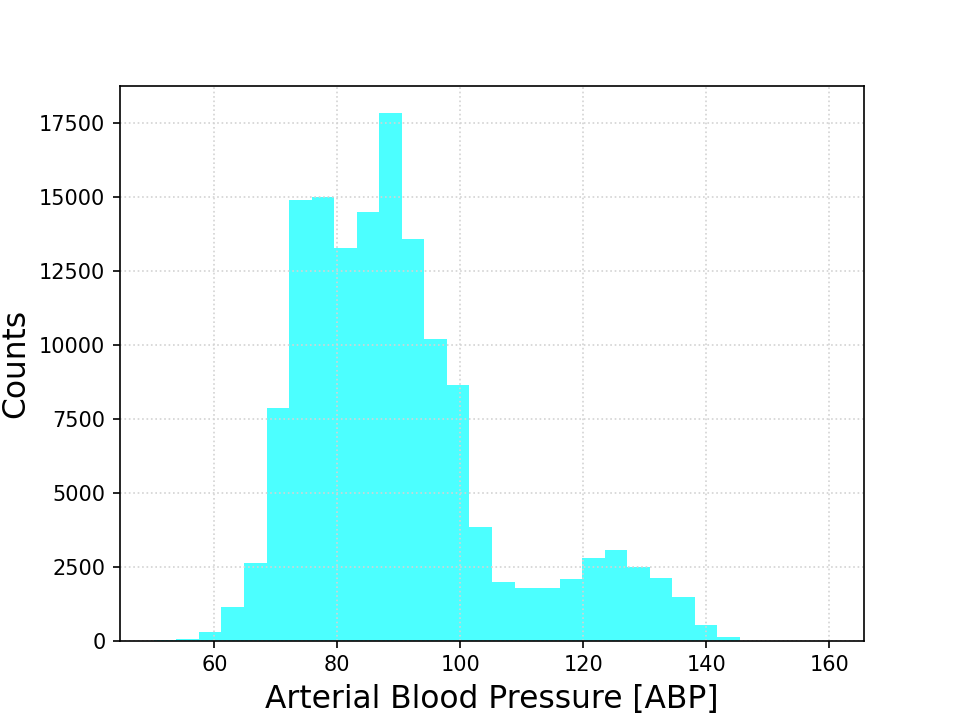
\includegraphics[width=\textwidth]{plots/histo_ABP.png}

	\end{minipage}
	\begin{minipage}[b]{0.32\textwidth}
		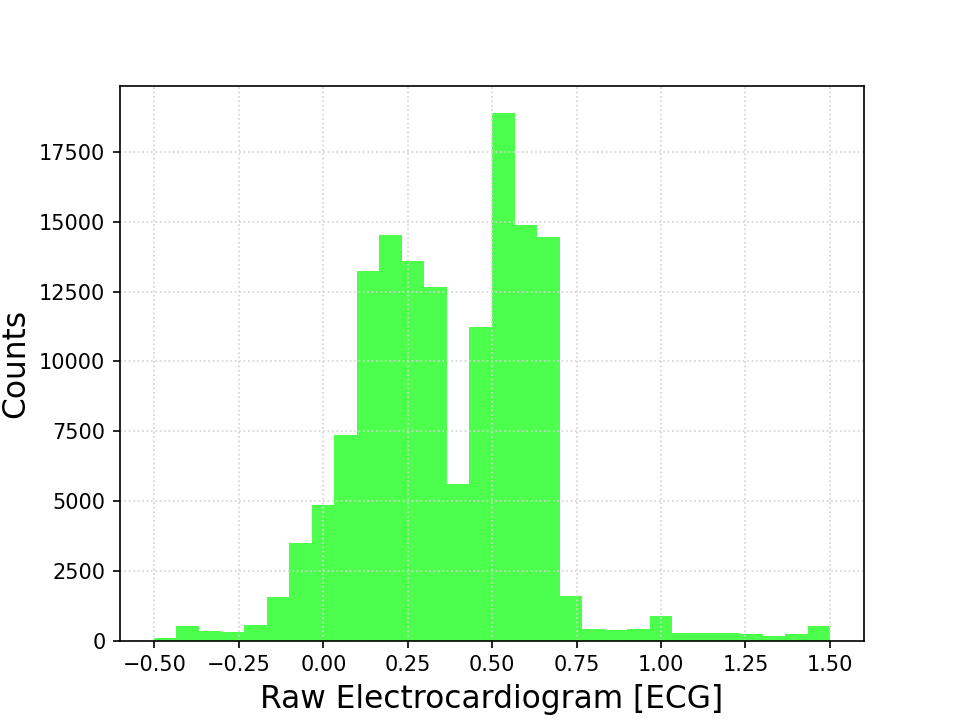
\includegraphics[width=\textwidth]{plots/histo_ECG.png}

	\end{minipage}
	\begin{minipage}[b]{0.32\textwidth}
		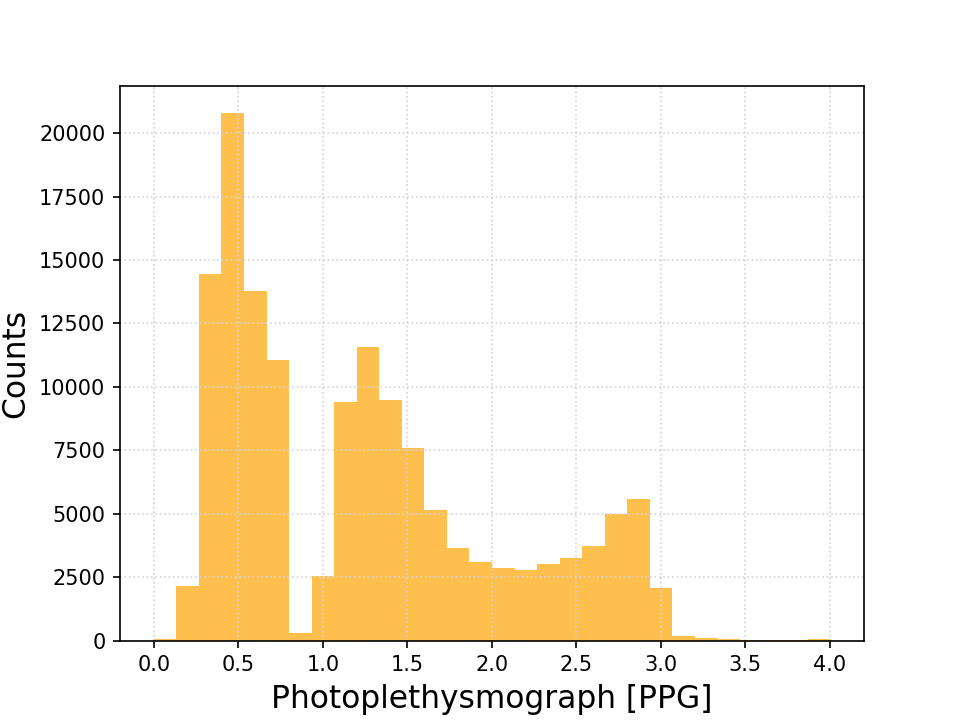
\includegraphics[width=\textwidth]{plots/histo_PPG.png}

	\end{minipage}
	\begin{minipage}[b]{0.32\textwidth}
		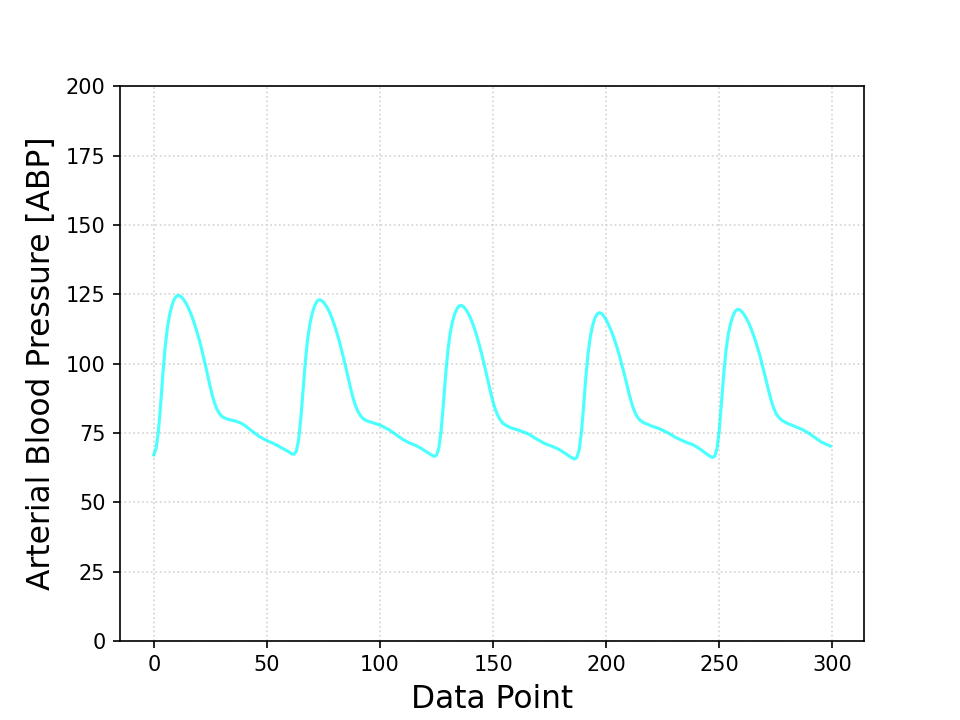
\includegraphics[width=\textwidth]{plots/series_ABP_zoom.png}

	\end{minipage}
	\begin{minipage}[b]{0.32\textwidth}
		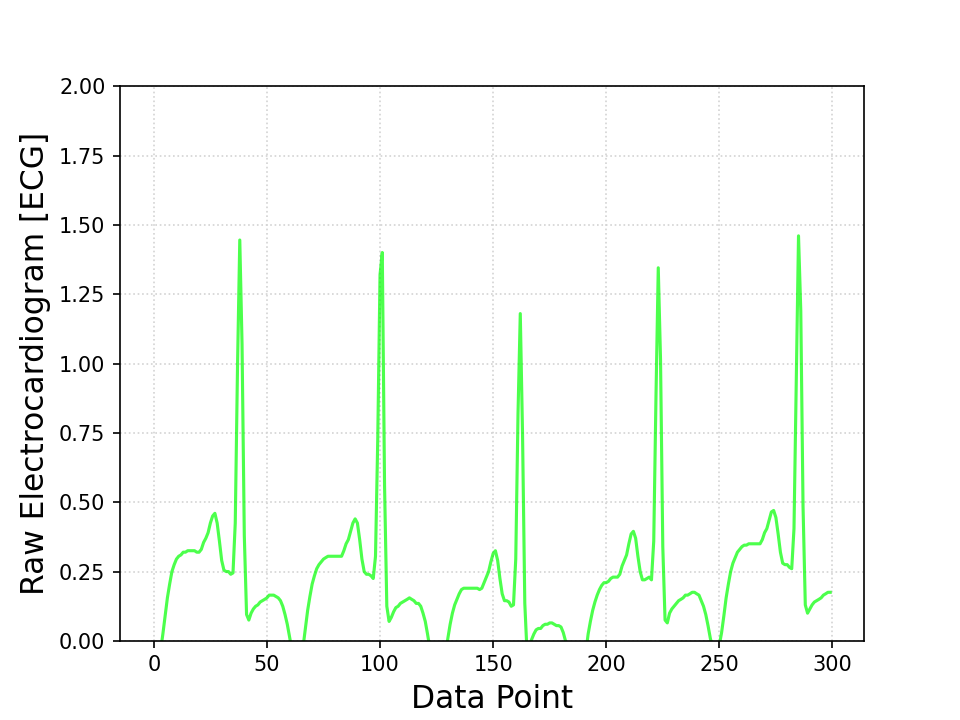
\includegraphics[width=\textwidth]{plots/series_ECG_zoom.png}

	\end{minipage}
	\begin{minipage}[b]{0.32\textwidth}
		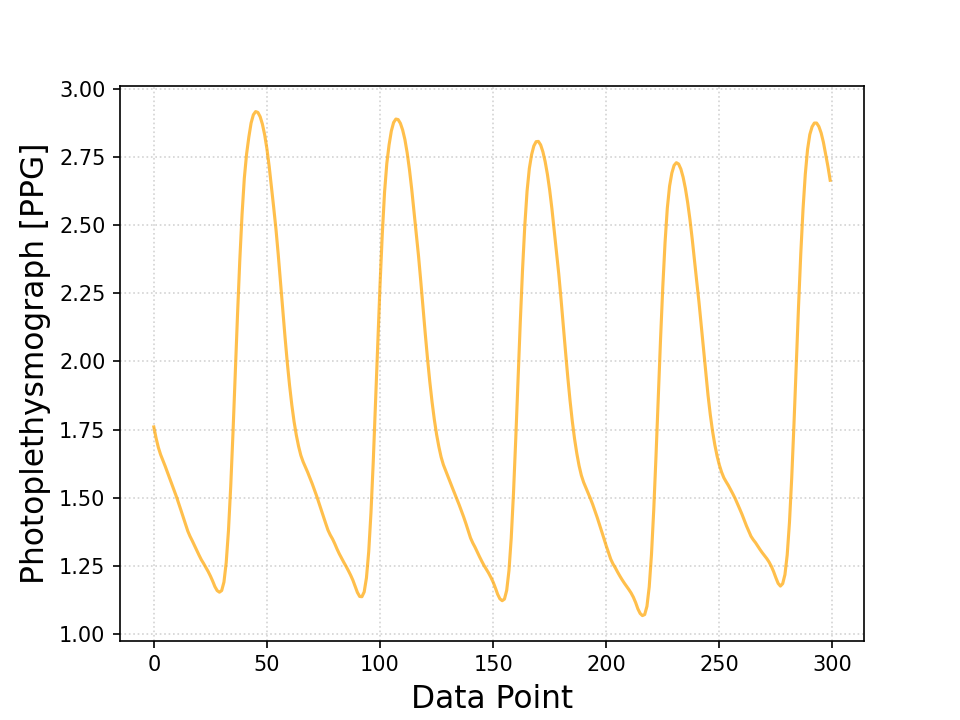
\includegraphics[width=\textwidth]{plots/series_PPG_zoom.png}
	\end{minipage}


	\caption{Distribution for the ABP, ECG and PPG signals.}
	\label{signals}
\end{figure}





\paragraph{Task}
\noindent This data set is our choice for the regression part with ABP being the target variable.
The most common approach to measure (BP) is by using a cuff, wrapped around the upper arm and inflated. A pressure sensor inserted in the cuff records the arterial pulsations during the cuff deflation, and the amplitudes of these pulsations are used to calculate systolic and diastolic BP. The limitations of the approach include that it relies on a set of empirical coefficients to map the pulse amplitudes to systolic and diastolic BP, specific to the used device. Furthermore, this kind of measurements in patients with atherosclerosis or obese patients, whose pulse amplitudes can be weak, are subject to large errors.

For these reasons, it is very interesting to study the possibility to study a regression model able to predict the BP by using the PPG and/or the ECG signals.





\section{Data Set: Drug Consumption}
This dataset \cite{fehrman2017factor} includes records of drug usage of 1885 respondents, together with attributes regarding personal information, collected through an online survey. Data refers to two general categories. 
The first is related to personal aspects of the respondent: level of education, age, gender, country of residence and ethnicity. Many studies have shown that personality traits such as neuroticism (N), extraversion (E), openness to experience (O), agreeableness (A), and conscientiousness (C) can be associated to drugs consumption. For example, the personality traits of N,E, and C are highly correlated with dangerous health behaviours. In this dataset, two additional personality traits are considered: the Barratt Impulsiveness Scale version 11 (BIS-11), and the Impulsivity Sensation-Seeking scale (ImpSS). The dataset include then the scores of these seven personality traits.

The second category of data regards the usage of specific drugs acting as central nervous system depressants, stimulants, or hallucinogens:alcohol, amphetamines, amyl nitrite, benzodiazepine, cannabis, chocolate, cocaine, caffeine, crack, ecstasy, heroin, ketamine, legal highs, LSD, methadone, mushrooms, nicotine and volatile substance abuse and one fictitious drug (Semeron) which was introduced to identify over-claimers. 

For each substance, the respondent had to classify the own usage using according to the following frequency categories: "Never Used", "Used over a Decade Ago", "Used in Last Decade", "Used in Last Year", "Used in Last Month", "Used in Last Week", and "Used in Last Day".



\clearpage
\paragraph{Dataset}

\noindent The data set contains xxx TO DO.

\begin{figure}[h!]
	\centering
	\begin{minipage}[b]{0.32\textwidth}
		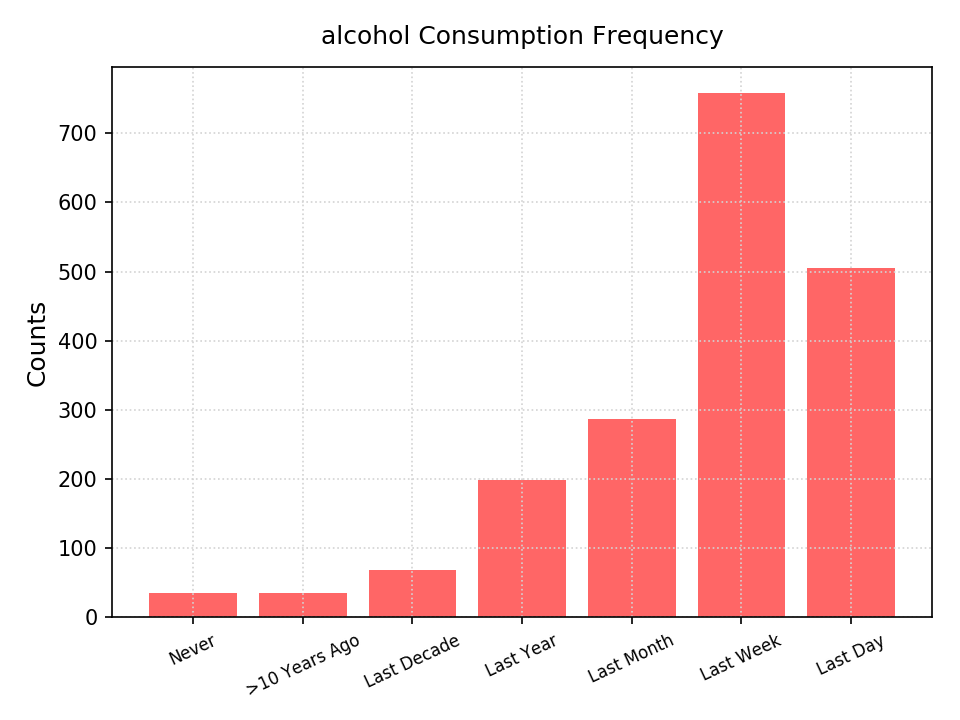
\includegraphics[width=\textwidth]{plots/drugsPlots/alcohol_freq.png}

	\end{minipage}
	\begin{minipage}[b]{0.32\textwidth}
		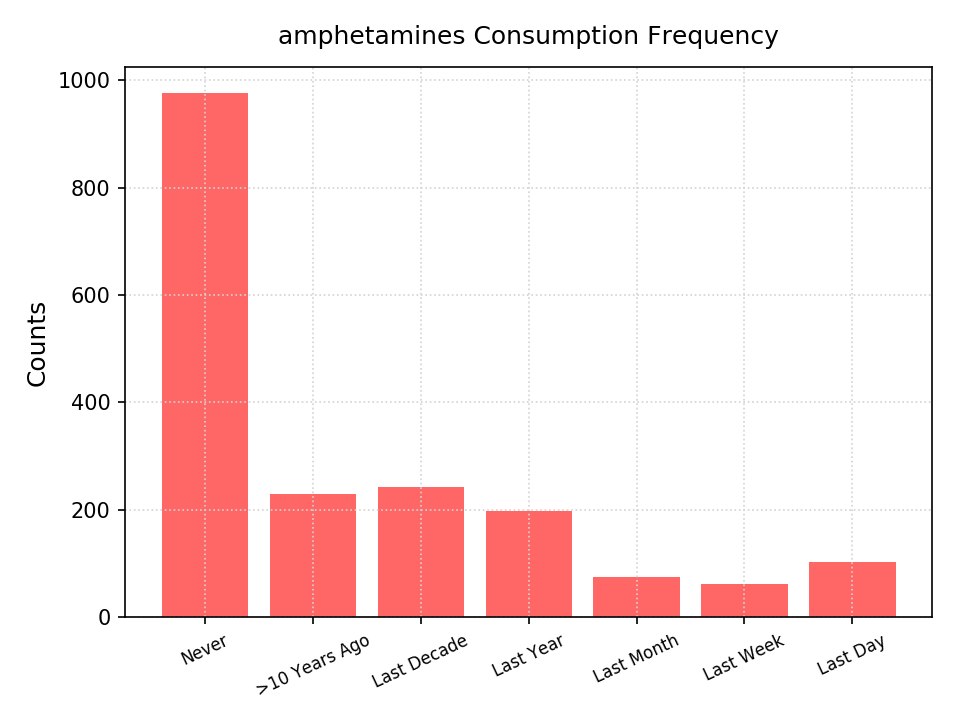
\includegraphics[width=\textwidth]{plots/drugsPlots/amphetamines_freq.png}

	\end{minipage}
	\begin{minipage}[b]{0.32\textwidth}
		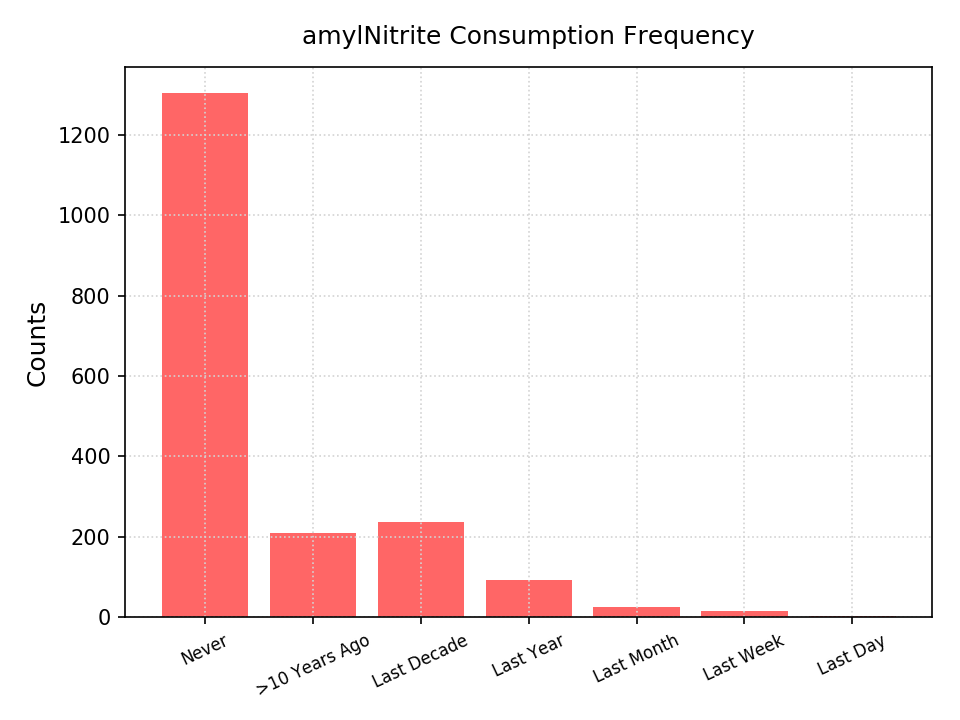
\includegraphics[width=\textwidth]{plots/drugsPlots/amylNitrite_freq.png}
	\end{minipage}
	\begin{minipage}[b]{0.32\textwidth}
	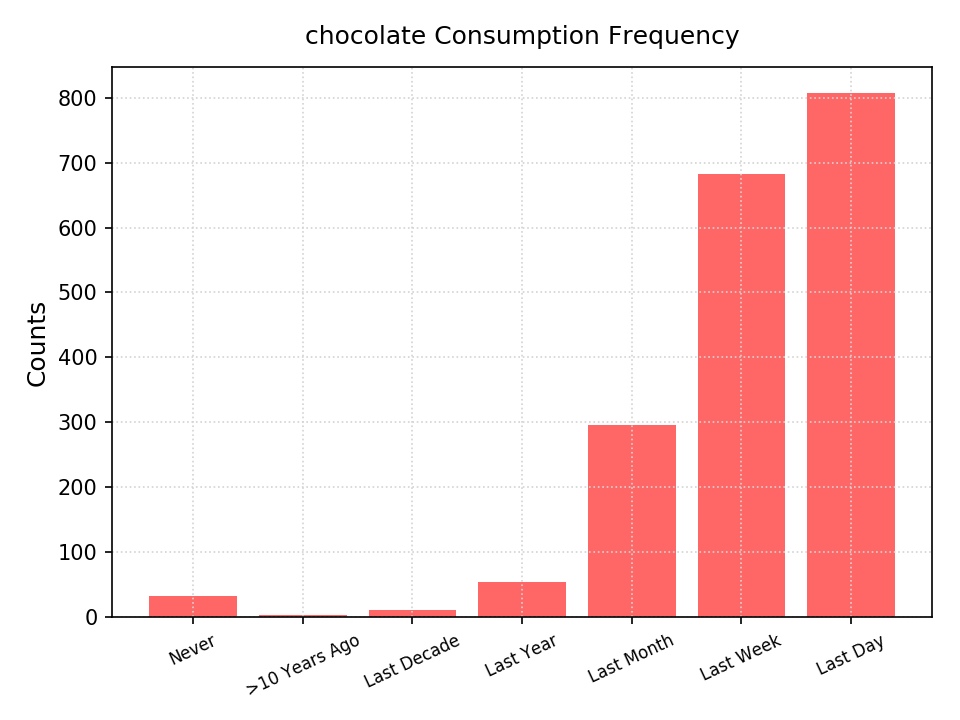
\includegraphics[width=\textwidth]{plots/drugsPlots/chocolate_freq.png}
	
\end{minipage}
\begin{minipage}[b]{0.32\textwidth}
	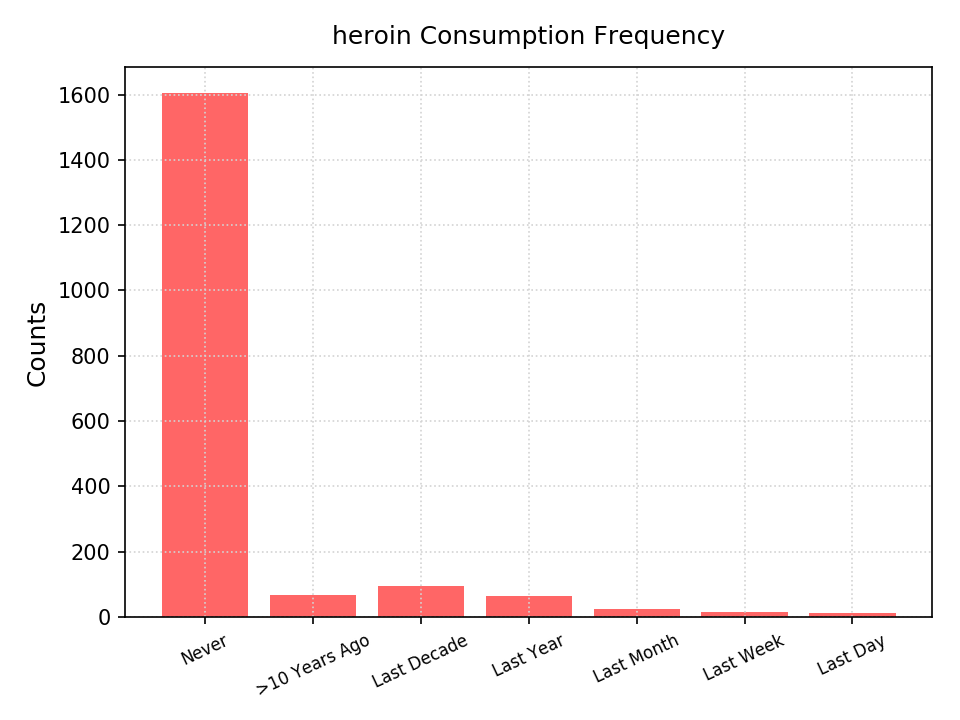
\includegraphics[width=\textwidth]{plots/drugsPlots/heroin_freq.png}
	
\end{minipage}
\begin{minipage}[b]{0.32\textwidth}
	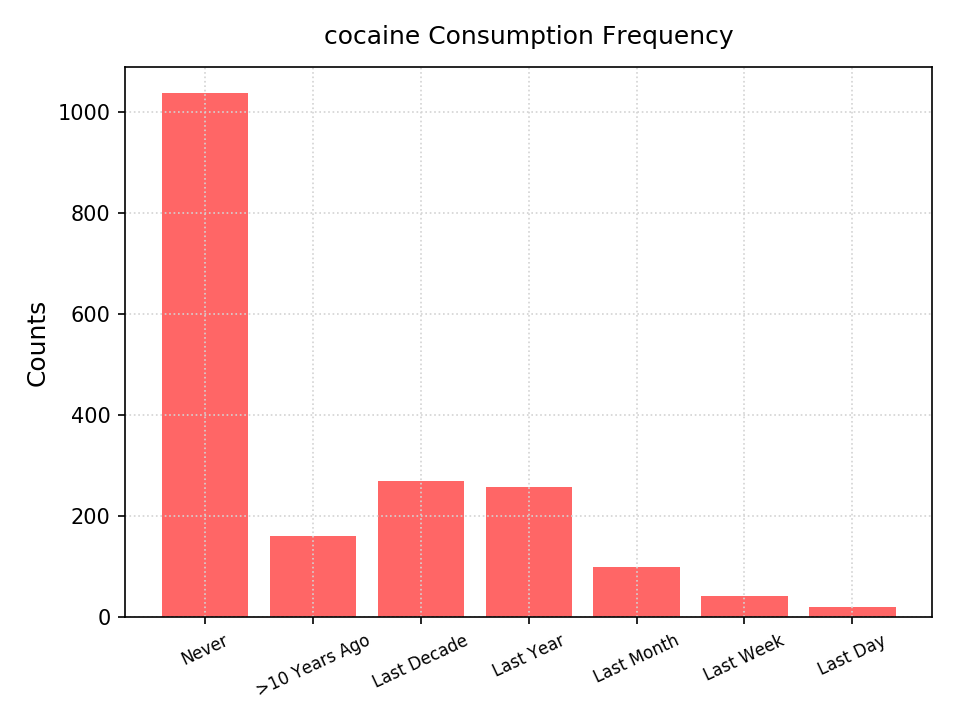
\includegraphics[width=\textwidth]{plots/drugsPlots/cocaine_freq.png}
\end{minipage}

	\caption{Example of frequency use for a selection of drugs.}
\label{drugs1}
\end{figure}


\begin{figure}[h!]
	\centering
	\begin{minipage}[b]{0.32\textwidth}
		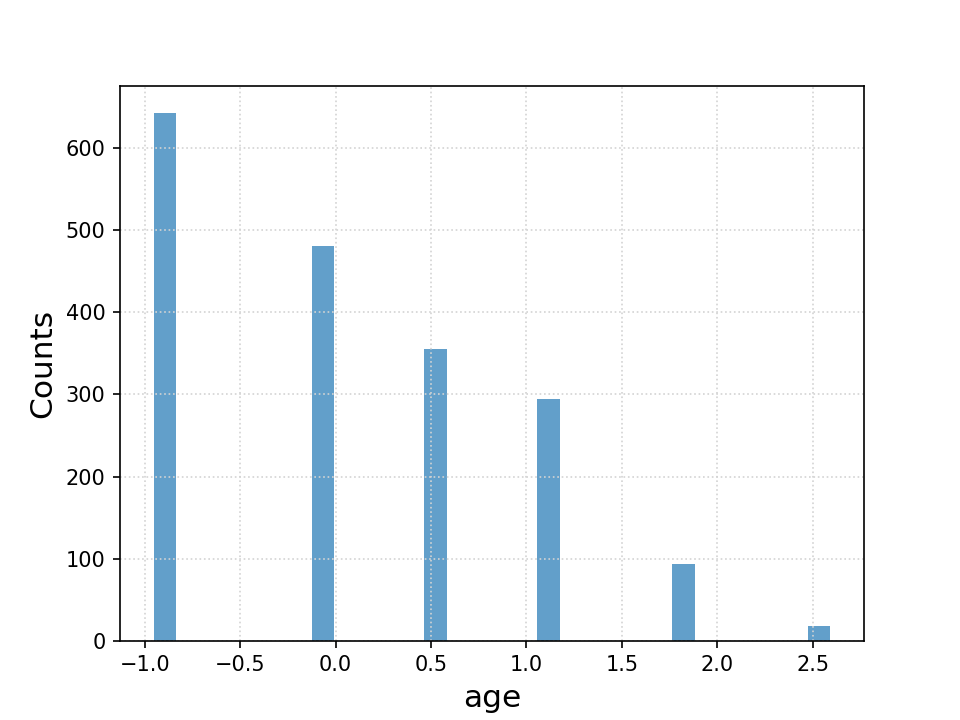
\includegraphics[width=\textwidth]{plots/drugsPlots/age.png}

	\end{minipage}
	\begin{minipage}[b]{0.32\textwidth}
		
\includegraphics[width=\textwidth]{plots/drugsPlots/country.png}

	\end{minipage}
	\begin{minipage}[b]{0.32\textwidth}
		
\includegraphics[width=\textwidth]{plots/drugsPlots/gender.png}
	\end{minipage}
	\caption{Distribution for drugs.}
	\label{drugs2}
\end{figure}
\begin{figure}[h!]
	\centering
	\begin{minipage}[b]{0.32\textwidth}
		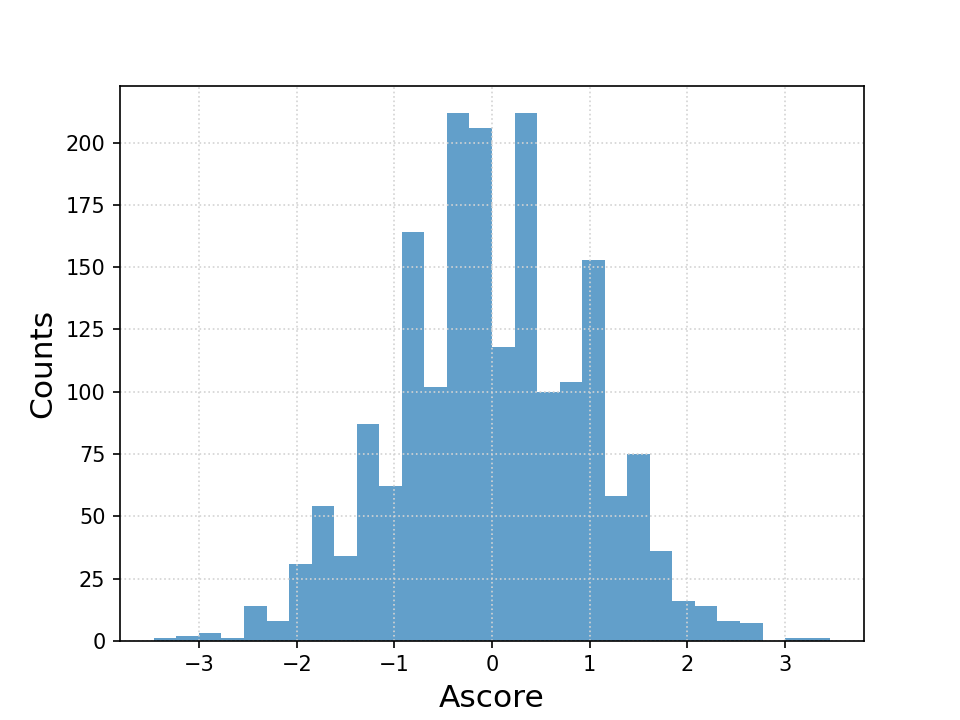
\includegraphics[width=\textwidth]{plots/drugsPlots/Ascore.png}

	\end{minipage}
	\begin{minipage}[b]{0.32\textwidth}
		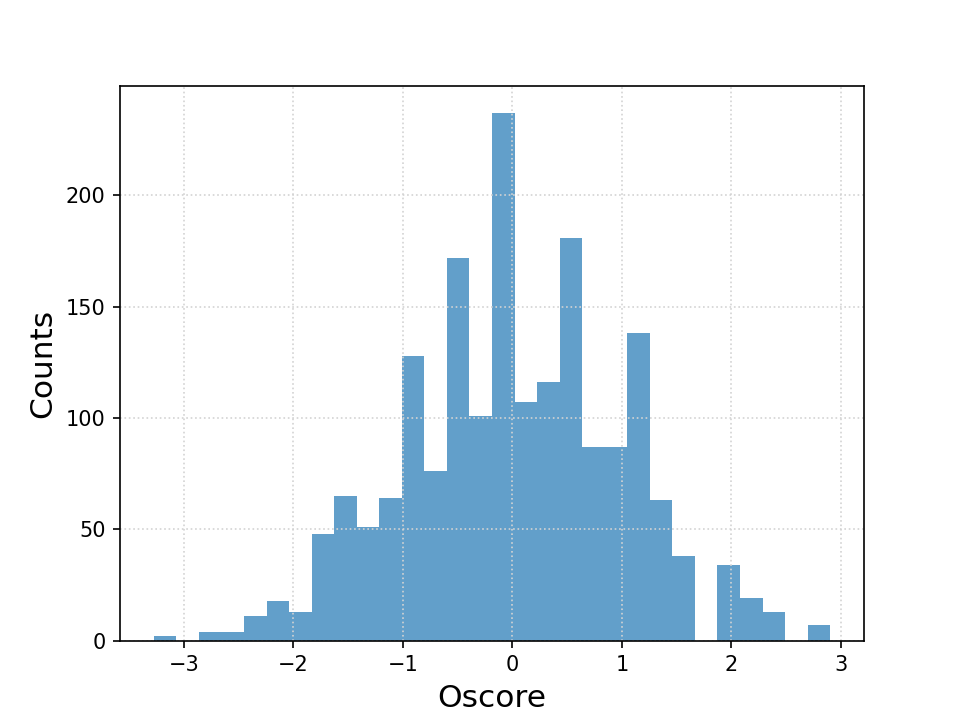
\includegraphics[width=\textwidth]{plots/drugsPlots/Oscore.png}

	\end{minipage}
	\begin{minipage}[b]{0.32\textwidth}
		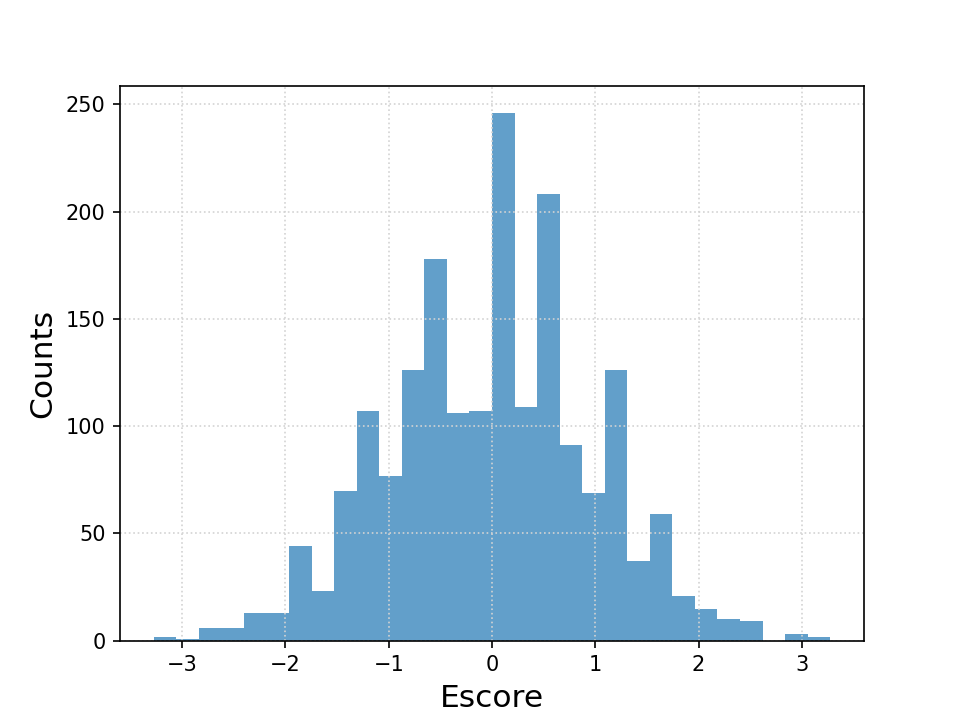
\includegraphics[width=\textwidth]{plots/drugsPlots/Escore.png}
	\end{minipage}
	\caption{Distribution for drugs.}
	\label{drugs3}
\end{figure}



\paragraph{Task}

This data set is very appropriate for classification experiments, given the partition of the data attributes into different classes.



\newpage
\bibliography{literature.bib}{}
\bibliographystyle{unsrt}

\end{document}
